This chapter describes the multicore implementation of the LM language,
including its compiler, supporting runtime and parallelism. We first start with
an overview of the implementation in order to understand how all pieces of the
implementation fit together. Secondly, we describe how parallelism is achieved,
including its data structures and thread scheduling. Thirdly, we present the
implementation details of coordination and how it relates with parallelism.  We
then describe the runtime and data structure used to implement nodes and the
database of facts, followed by the compilation algorithm used by our compiler to
turn logical rules into efficient C++ code.

\section{Overview}
The implementation of LM is composed of a compiler and a virtual machine~(VM).
Figure~\ref{fig:implementation:overview} presents an overview of the compilation
process for LM programs. The two main boxes represent the two major components
of the system, namely, the compiler and virtual machine.

\begin{figure}[ht]
  \centering
  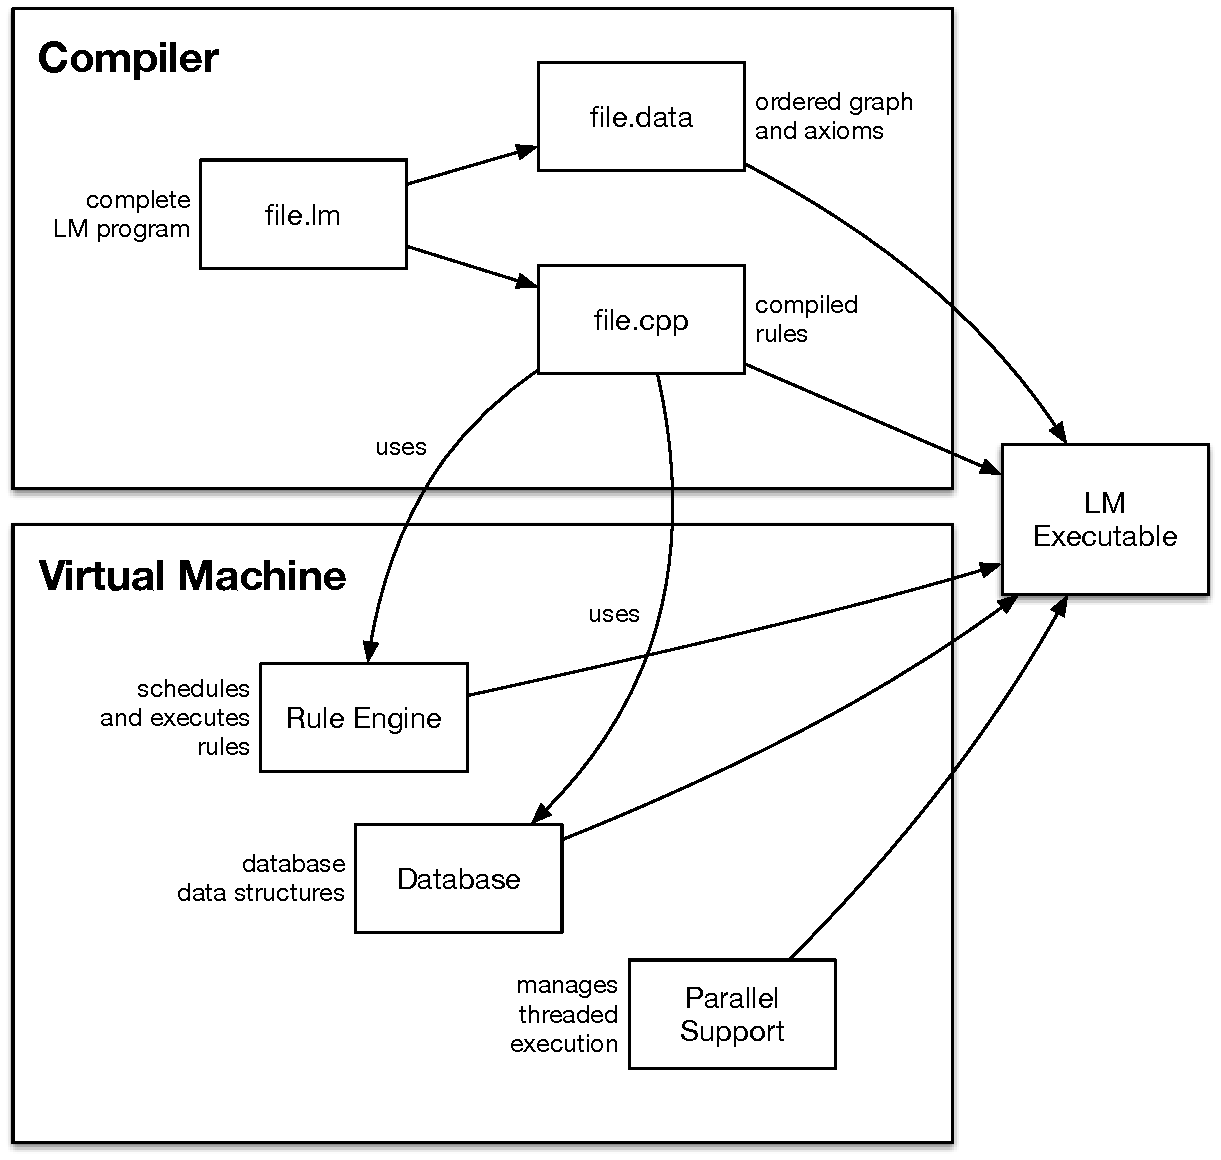
\includegraphics[width=.75\linewidth]{figures/implementation/overview.pdf}
  \caption{Compilation of a LM program into an executable. The compiler
     transforms a LM program into \code{file.cpp}, C++ file with compiled
     rules, and a \code{data} file with the graph structure and initial facts. The virtual
     machine which includes code for managing multithreaded execution and the
     database of facts is then linked with \code{file.cpp} to create a
     standalone executable that can be run in parallel.}
  \label{fig:implementation:overview}
\end{figure}

The virtual machine contains supporting data structures for managing the
database of facts and to schedule the execution of rules. The parallel engine is
also a major part of the virtual machine and is responsible for managing
multithreaded execution by launching threads, managing communication and
and scheduling parallel execution, including coordination.

The compiler transforms LM files into C++ code that use the virtual machine
facilities to implement the program logic.  The compiled code implements the
inference rules of the program and uses the API of the virtual machine to derive
and retract facts and to schedule the execution of rules.  The compiler also
creates a separate file, named \code{file.data}, with the program's initial
facts and graph structure. The graph structure is reconstructed in parallel once
the program starts.

To complete the compilation process, we use a C++ compiler to compile the
virtual machine files and \code{file.cpp} into object files that are then
linked along with \code{file.data}. At the end, we have a standalone
executable that allows the user to input the number of threads to use,
scheduling strategies (i.e., disable coordination), run time measurement
facilities and also database printing facilities.

Alternatively, the programmer may also decide to compile a more general version
of the virtual machine that is able to run byte-code files generated by the
compiler. This allows faster development since the programmer only needs to
recompile the LM program and not the whole stack. However, LM programs will run
slower since the byte-code must be interpreted by the virtual machine. This
severely affects programs with many mathematical operations, especially floating
point computations.

\iffalse
\subsection{Graph Clustering}

The graph structure stored in file \code{file.data} is constructed by the
compiler by analyzing the program's initial facts and then ordering the nodes of
the graph.  In order to distribute computation across threads it is important to
increase locality of communication, so that a node makes most of its
communication to neighbor nodes that are being handled by the same thread. The
graph structure in \code{file.data} is written in order to improve locality and
reduce communication between threads.

The compiler analyzes the node address constants (that are prepended by the
symbol @) and the initial facts of the program. After parsing and type-checking the
program code, the compiler then optimizes the topology by building an internal
representation of the graph.  In this phase, each node address $a$ is mapped
using a function $M(x)$ to a normalized node address $n$. Function $M(x)$ is
bijective and the domain is the set of all nodes described in the source code.
The co-domain of $M$ is the discrete interval $[0, N[$, where $N$ is the number
of nodes in the graph. The byte-code of a LM program includes all the pairs $(x,
M(x))$ so that the runtime system can put this information to use.

We have three methods for defining the function $M(x)$:

\begin{itemize}
   \item \emph{Static}: the compiler uses the node addresses presented in the
      code as long as they fill the discrete interval $[0, N[$.
   \item \emph{Randomized}: the mapping is done randomly.
   \item \emph{Breadth-First}: the mapping is built by picking an arbitrary node, $n_{zero}$
   and setting $M(n_{zero}) = 0$, then we select all neighbors of $n_{zero}$ and start defining
   their mappings in increasing order, $1, \dotsc, N-1$, and adding its neighbors for later processing
   in a breadth first fashion.
\end{itemize}

The breadth-first method is used with the intent of clustering closer nodes in
an ordered fashion.  While not optimal, using a breadth-first approach is very
efficient and has good results for irregular graphs. If we use a static division
of work between $N$ threads, where each thread is responsible to process a
pre-defined set of nodes, we can efficiently slice the codomain of function
$M(x)$ and divide it between the $N$ threads.

For an example, consider the graph in Fig.~\ref{fig:compiler:topology1}. The
node addresses represented are the ones included in the source code. Using a
breadth-first method starting by node 1, we get the following order: 1, 2, 3, 7,
5, 6 and 4. If we had to do a static division with 2 threads, thread 1 would get
1, 2, 3, 7 and thread 2 would get 5, 6 and 4. Note from
Fig.~\ref{fig:compiler:topology1} that only 3 edges exist between the nodes of
thread 1 and thread 2. This greatly reduces communication between threads and
improves parallel efficiency.

\begin{figure}[ht]
  \centering
  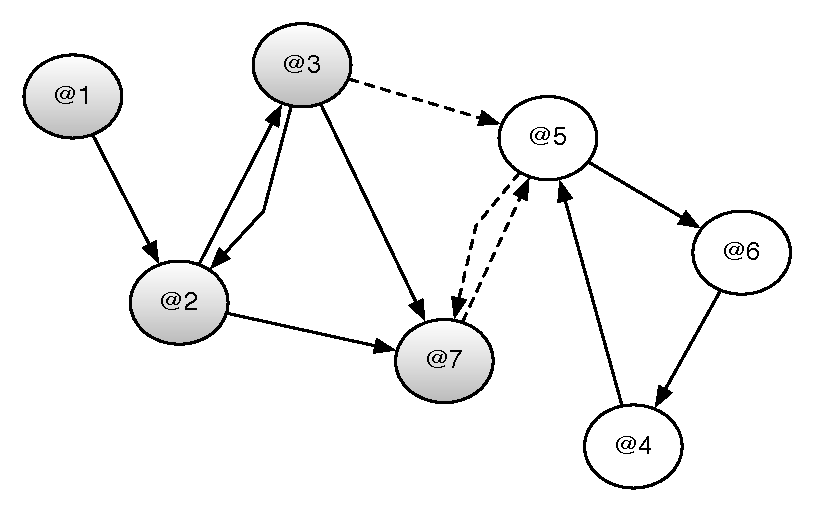
\includegraphics[width=0.6\textwidth]{figures/compiler/topology1.pdf}
  \caption{Topology using a breadth-first method.}
  \label{fig:compiler:topology1}
\end{figure}
\fi


\section{Parallelism}
A key goal of our parallel design is to keep the threads as busy as possible and
to reduce inter-thread communication. Initially, the VM partitions the
application graph of $N$ nodes into $T$ subgraphs (the number of threads) and
then each thread will work on their own subgraph.  During execution, threads can
steal nodes of other threads to keep themselves busy. The load balancing aspect
of the system is performed by our work scheduler that is based on a simple work
stealing algorithm. The pseudo-code for the main thread loop is shown in
Fig.~\ref{alg:thread_work_loop}. In each round, a thread inspects its work queue
for \emph{active nodes}, which are nodes with new candidate rules and, if there
is any, procedure \texttt{process\_node()} performs computation at the node
level. If the work queue is empty, the thread attempts to steal half of the
nodes from another thread. Starting from a random thread, it cycles through all
the threads to find one active thread. Eventually, there will be no more work to
do and the threads will go idle. There is a global atomic counter, a global
boolean flag and one state flag for each thread that are used to detect
termination. Once a thread goes idle, it decrements the global counter and
changes its flag to idle. If the counter reaches zero, the global flag is set to
idle. Since every thread will be busy-waiting and checking the global flag, they
will detect the change and stop executing.

\begin{figure}
\begin{algorithm}[H]
   \KwData{Thread TH, THREADS}
   \While{true}{
      $node \longleftarrow TH.work\_queue.pop\_node()$ \;
      \uIf{$node$}{
         $TH.process\_node(node)$\;
      }
      \Else{
         \tcc{Need to steal some nodes.}
         $target \longleftarrow random(len(THREADS))$\;
         $i \longleftarrow 0$\;
         \For{$i < len(THREADS)$}{
            $target \longleftarrow (target + 1) \% len(THREADS)$\;
            $nodes = THREADS[target].steal\_half()$\;
            \If{$len(nodes) > 0$}{
               $TH.work\_queue.add\_to\_queue(nodes)$\;
               break\;
            }
            $i \longleftarrow i + 1$\;
         }
         \If{$len(TH.work\_queue) == 0$}{
            \tcc{try to terminate}
            $TH.become\_idle()$\;
            \If{$TH.synchronize\_termination()$}{
               \Return{}\;
            }
            \tcc{There's new nodes in the queue.}
            $TH.become\_active()$\;
         }
      }
 }
\end{algorithm}
\caption{Thread work loop: threads process active nodes from the work queue
   until no more active nodes are available. Node stealing using a \emph{steal
      half} strategy is employed when the thread has no more active nodes.}
 \label{alg:thread_work_loop}
\end{figure}

Figure~\ref{fig:implementation:vm_overview} presents the layout of our virtual
machine for a program with six nodes and two running threads. Each thread space
includes the nodes owned by the thread (the dotted arrows represent the edges
between nodes) and a \emph{Work Queue}, which contains \emph{active nodes},
i.e., nodes that have new facts to process, and can be implemented as a simple
linked list. Initially, the \emph{Work Queue} is filled with all the nodes of
the thread in order to derive the initial facts.
Figure~\ref{fig:implementation:vm_overview} also illustrates the internal
structure layout of a node, which includes: the database of linear facts
(\emph{Linear DB}); the database of persistent facts (\emph{Persistent DB}); the
rule matching structures (\emph{Rule Engine}); and an auxiliary buffer for
storing intermediate facts coming from other threads (\emph{Fact Buffer}).

\begin{figure*}[t]
\centering
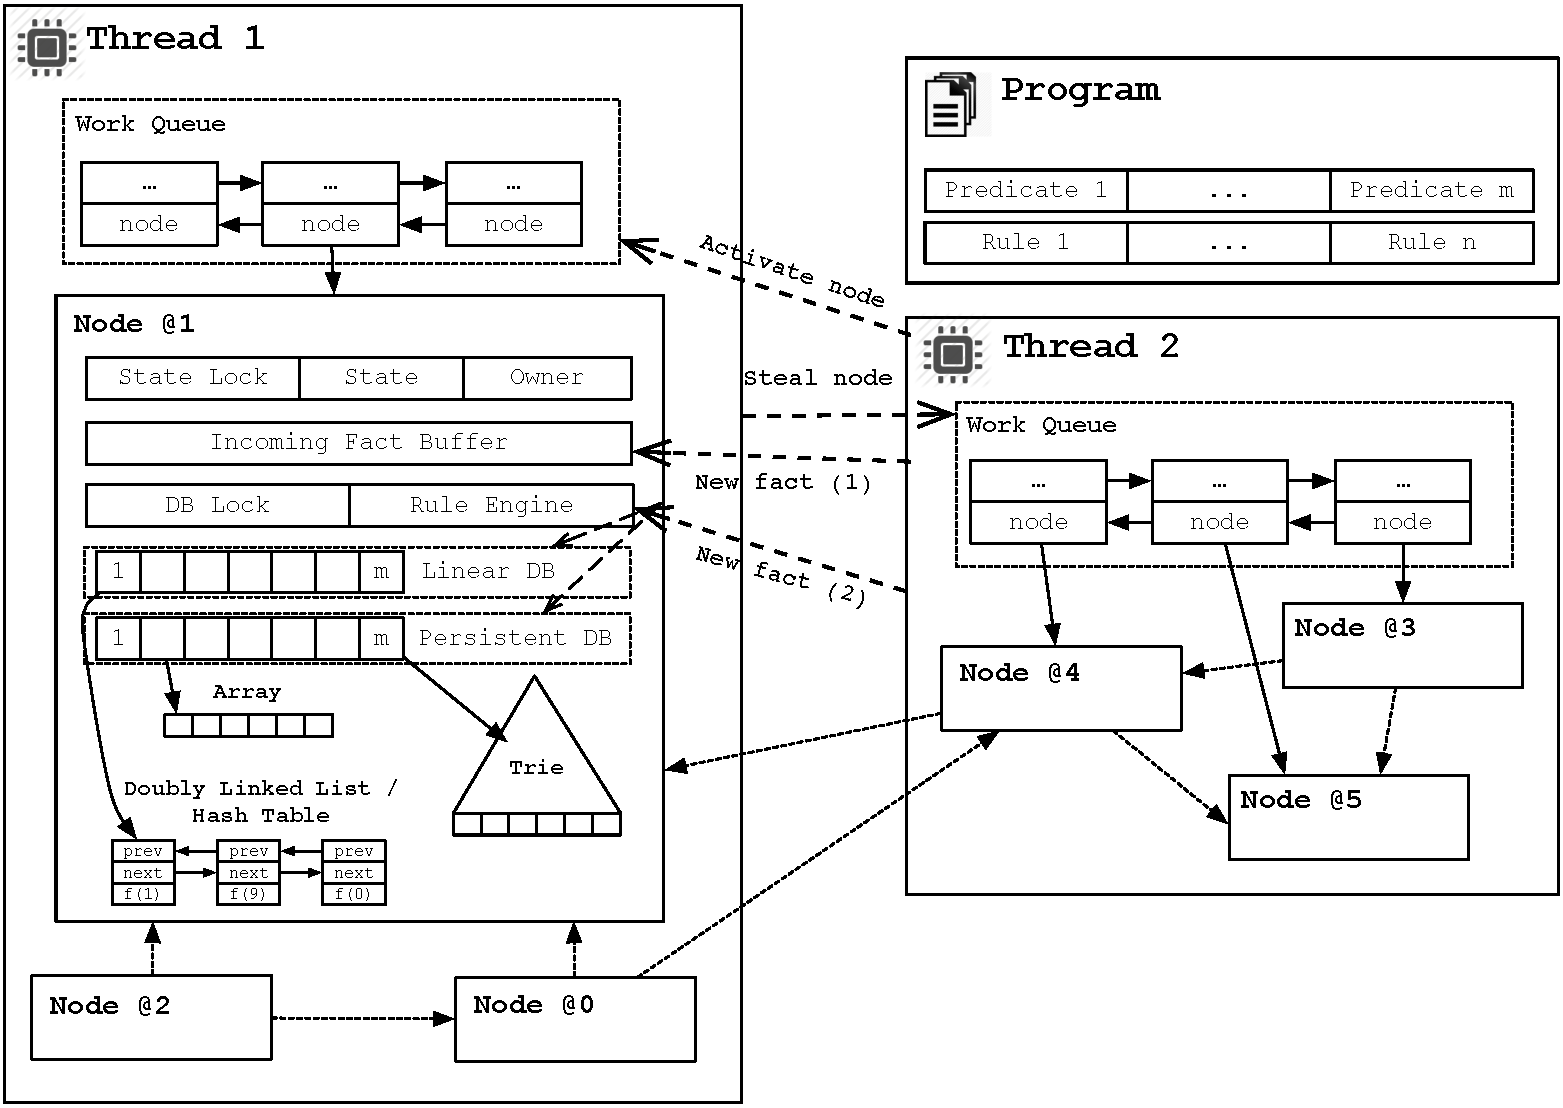
\includegraphics[width=\textwidth]{figures/implementation/vm_overview.pdf}
\caption{Layout of the virtual machine. Each thread has a work queue that
   contains active nodes (nodes with facts to process) that are processed one
   by one by the thread. Communication between threads happens when nodes
   send facts to nodes located in other threads.}
\label{fig:implementation:vm_overview}
\end{figure*}

Whenever a new fact is derived through rule derivation, we need to update the
data structures for the corresponding node. This is trivial if the thread that
derived the fact also owns the node. If that is not the case, then we have to
synchronize since multiple threads might be updating the same node's data
structures. We added a lock and a boolean flag to each node to protect the
access to its data structures. When the flag is activated, it means that the
node is currently being executed by the owning thread. For example, in
Fig.~\ref{fig:implementation:vm_overview}, if thread 2 derives a fact to node
\texttt{@1} (owned by thread 1), then thread 2 checks the node's flag and if not
activated, will lock node \texttt{@1} and perform the required updates
(\emph{New fact (1)}). If the flag is activated, it will not touch the main node
data structures, but instead will add the new fact to \emph{Fact Buffer}
(\emph{New fact (2)}). The facts stored in \emph{Fact Buffer} will then be
processed whenever the corresponding node's flag becomes active.

There is another thread interaction that might happen during fact derivation if
the node receiving a new fact is not active. In such case, the sending thread
needs to activate the node by pushing it to the \emph{Work Queue} of the target
thread. For example, consider again the situation in which thread 2 sends a new
fact to node \texttt{@1}. If node \texttt{@1} is not active, then thread 2 also
needs to activate \code{@1} by pushing it to the \emph{Work Queue} of thread 1.
After this synchronization point, the target thread is ensured to be active and
with a new node to process.

\subsection{Runtime Data Structures And Garbage Collection}

LM supports recursive types such as lists, arrays and structures. These compound
data structures are immutable and shared between multiple facts. Such structures
are stored in the heap of the VM and are managed through reference counting. For
instance, each list is a \emph{cons cell} with 3 fields: \texttt{tail}, the
pointer to the next element of the list; \texttt{head}, the element stored by
this element of the list; and \texttt{refs}, which counts the number of pointers
to this list element in the VM. The list is deleted from the heap whenever
\texttt{refs} is decremented to zero.

Nodes are also subject to garbage collection. If the database of a node becomes
empty and there are no references to the node from other logical facts, then the
node is deleted from the program. We keep around a small number of freed nodes
that can be reused immediately if another node is created.  We avoid garbage
collection schemes based on tracing since objects are created and discarded in
very specific points of the virtual machine and the runtime objects cannot
contain circular references. A reference counting mechanism is thus more
appropriate than a parallel tracing garbage collector which would entail pausing
the execution of the program to garbage collect all the unused objects.


\section{Coordination}
In order to support priorities and node partitioning, we extended the work queue
of each thread, as presented in Fig.~\ref{fig:implementation:vm_overview}, to
include two new pairs of queues: two doubly linked lists known as the
\emph{standard queue} and two min/max heaps known as the \emph{priority queue}.
The standard queue contains nodes without priorities and supports push into
tail, remove node from the head, remove arbitrary node, and remove first half of
nodes.  The priority queue contains nodes with priorities and is implemented as
a binary heap array.  It supports the following operations: push into the heap,
remove the \emph{min} node, remove an arbitrary node, remove half of the nodes
(vertical split), and priority update.  Operations for removing half of the
queue are implemented in order to support node stealing, while operations to
remove arbitrary nodes or update priority allows threads to change the priority
of nodes.  Table~\ref{fig:implementation:table_queue} shows the complexity of
queue operations and compares the standard queue against the priority queue.
Except for the remove half operation, priority queue operations are more
expensive.

\begin{table}[h]
   \begin{tabular}{| c | c | c |}
      \hline
      \textbf{Operation} & \textbf{Standard queue} & \textbf{Priority Queue} \\
      \hline
      Push & $\mathcal{O}(1)$ & $\mathcal{O}(\log{N})$ \\ \hline
      Pop & $\mathcal{O}(1)$ & $\mathcal{O}(\log{N})$ \\ \hline
      Remove & $\mathcal{O}(1)$ & $\mathcal{O}(\log{N})$ \\ \hline
      Remove Half & $\mathcal{O}(N)$ & $\mathcal{O}(\log{N})$ \\ \hline
      Priority Update & - & $\mathcal{O}(\log{N})$ \\ \hline
   \end{tabular}
   \caption{Complexity of queue operations for both the standard
      queue and the priority queue.}
   \label{fig:implementation:table_queue}
\end{table}

\begin{figure*}[t]
\centering
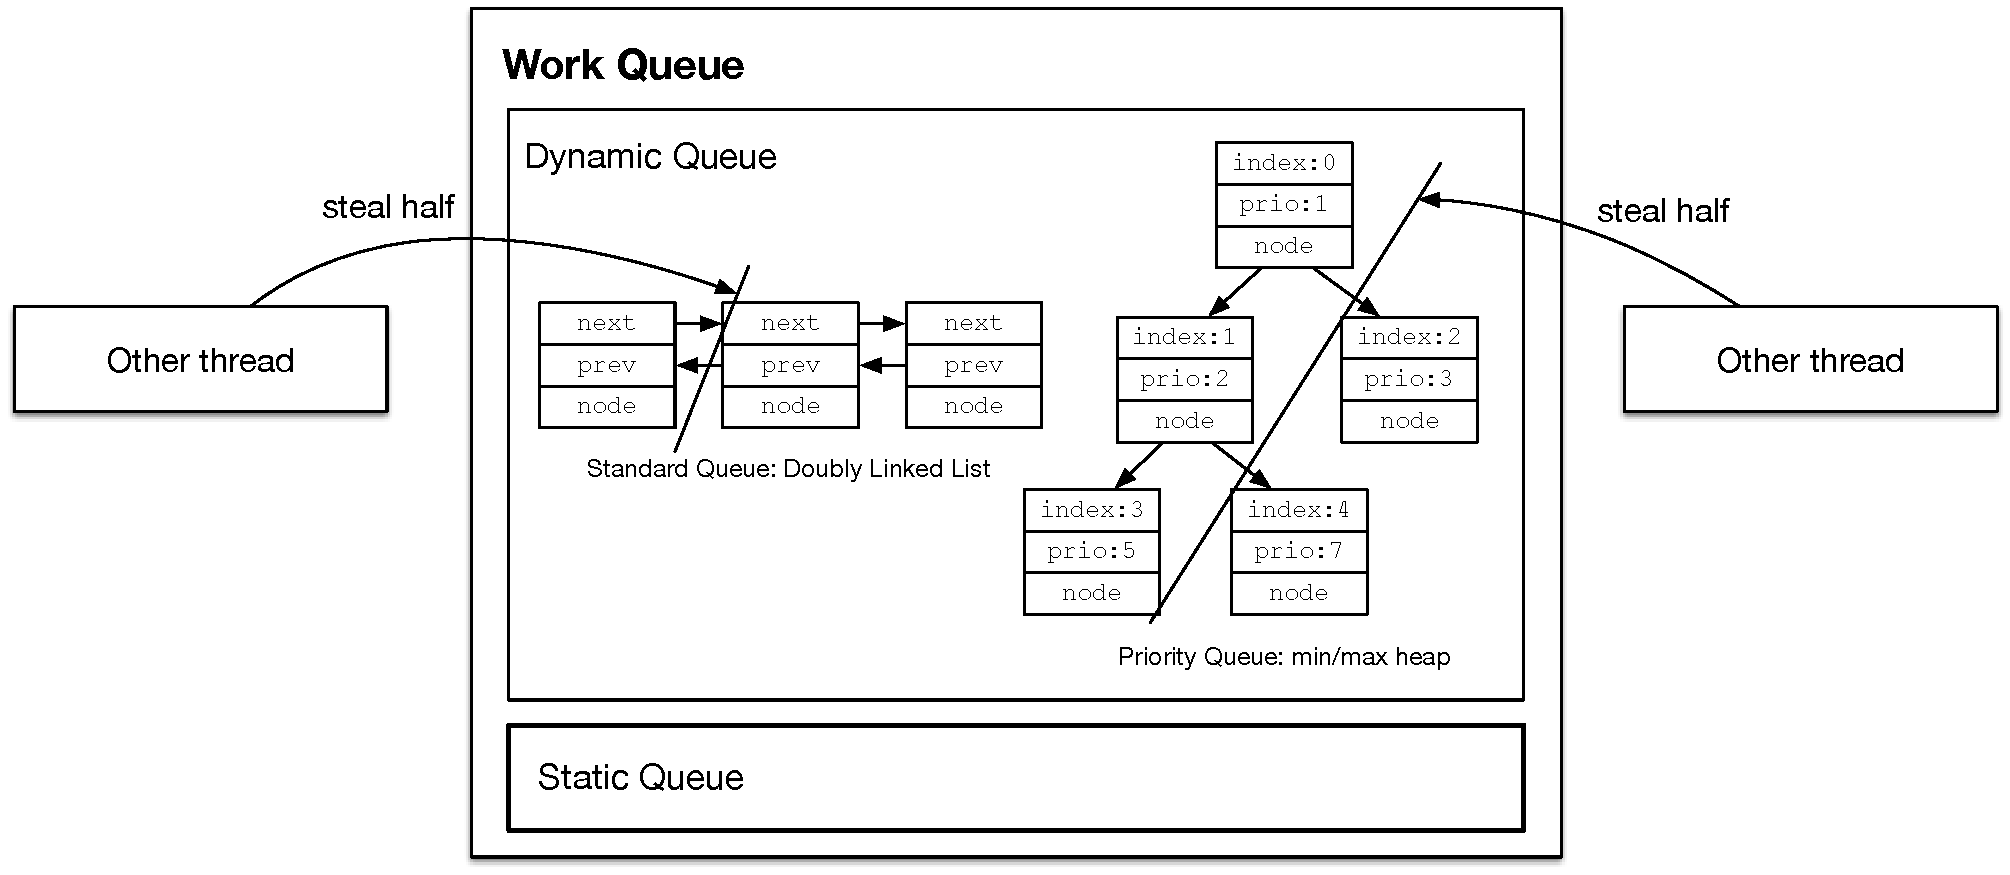
\includegraphics[width=0.95\textwidth]{figures/implementation/work_queue.pdf}
\caption{Thread's work queue and its interaction with other threads: the dynamic queue contains nodes that can be
   stolen while the static queue contains nodes that cannot be stolen. Both
   queues are implemented with one standard queue and one priority queue.}
\label{fig:implementation:work_queue}
\end{figure*}

The \texttt{next} and \texttt{prev} pointers of the standard queue are part of
the node structure in order to save space. These pointers are also used in the
priority queue but for storing the current priority and the index in the binary
heap array. Both the standard and priority queue are implemented as a pair of
queues. This first queue of each pair is a \emph{static queue} which contains
nodes that cannot be stolen and the second queue is the \emph{dynamic queue}
which contains nodes which can be stolen by other threads.
Figure~\ref{fig:implementation:work_queue} presents an overview of the two pairs
of queues and how the remove half operations are implemented in both queues in
order to support node stealing.  In the regular queue, the first $n/2$ elements
are removed from the front of the list and, in the priority queue, the binary
heap is split vertically for improved distribution of priorities.

Remember that to minimize inter-thread communication, node priorities are
implemented at the thread level, i.e., when a thread picks the highest priority
node from the priority queue, it picks the highest priority node from its
subgraph of nodes and not the highest priority node from the whole graph.

\subsection{Node State Machine}\label{sec:node_state_machine}

To accommodate the new coordination facilities, we added a new node state to the
state machine presented previously in Fig.~\ref{fig:local:node_states}.
Figure~\ref{fig:implementation:node_states} reviews the new set of states of
the state machine.

\begin{itemize}
   \item \textbf{running}: The node is deriving rules.
   \item \textbf{inactive}: The node is inactive, i.e., it has no new facts and
      it is not in any
   queue for processing.
   \item \textbf{active}: The node has new facts and it is in some queue waiting
   to be processed.
   \item \textbf{stealing}: The node has just been stolen and it is in the process of being
   moved to another thread.
   \item \textbf{coordinating}: The node moves from one queue to another or
      inside the priority queue when changing its priority.
\end{itemize}

\begin{figure}[ht]
   \centering
   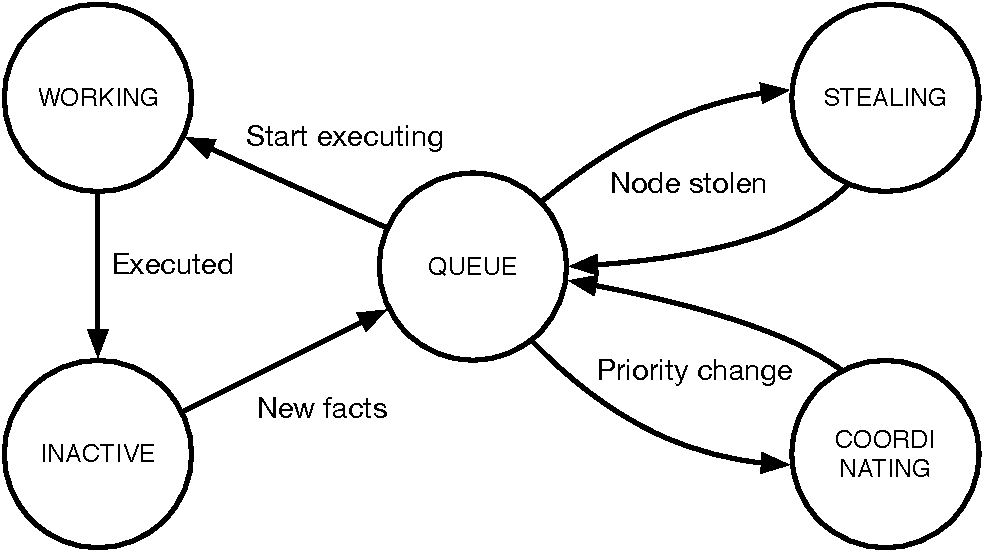
\includegraphics[width=0.55\textwidth]{figures/implementation/node_states.pdf}
   \caption{Node state machine extended with the new \textbf{coordinating}
   state.}
   \label{fig:implementation:node_states}
\end{figure}

\subsection{Coordination Instructions}\label{section:coordination:coord_instrs}

Coordination facts are implemented as API calls to the virtual machine which
implement the appropriate operations. Sensing facts read information about the
state of the virtual machine while action facts lock and update the appropriate
underlying data structures such as the node data structure or the thread's
queues.

When a thread $T_1$ performs coordination operations to a node owned by a thread
$T_2$, it needs to synchronize with $T_2$ and for that the \emph{State Lock} in
the target node needs to be acquired. Optionally, we may need to also lock the
queues of the thread $T_2$ if the priority is being updated or the queues of
thread $T_1$, if the node is moving to thread $T_1$. Note that both the standard
queue and priority queue have separate locks in order to allow concurrent
manipulation of the two data structures.

For the coordination facts \code{set-priority} and \code{add-priority}, when
multiple operations are directed to the same node during a single node
execution, we coalesce the multiple operations into a single operation.  As an
example, if a node derives two \code{set-priority} facts that change the
priority of node \code{@1} to \code{1} and \code{2}, the virtual machine
coalesces the two instructions into a single \code{set-priority} that is applied
with value \code{2} (the higher priority) after all the candidate rules of the
node are executed. The reason for this optimization is that nodes may run for
some number of steps during the lifetime of the program, therefore immediately
applying each and every coordination instruction is not cost effective. We aim
to reduce the amount of locking and movement of nodes inside the queues due to
priority updates.


\section{Node Data Structure}\label{sec:data_structures}
The main characteristic of LM rules is that they are constrained by the first
argument\footnote{In the implementation, the first argument of each fact is not
   stored.}. As shown in Fig.~\ref{fig:implementation:vm_overview}, each node
has its own database of linear facts (\emph{Linear DB}) and a database of
persistent facts (\emph{Persistent DB}).  Moreover, since only one thread at a
time will be using a node's database, we do not need to deal with
synchronization issues.

The databases of facts must be implemented efficiently because during matching
of rules we need to restrict the facts using \emph{join constraints}, which fix
arguments of predicates to instantiated values. Each node's database is
implemented using three kinds of data structures:

\begin{itemize}

\item \emph{Trie Data Structures} are used exclusively to store persistent
   facts. Tries are trees where facts are indexed by common prefix arguments.

\item \emph{Doubly Linked List Data Structures} are used to store linear facts.
   We use a double linked list because it is a very efficient way to add and
   remove facts.

\item \emph{Hash Table Data Structures} are used to improve lookup when linked
   lists are too long and when we need to do search filtered by a fixed
   argument. The virtual machine decides which arguments are best to be indexed
   (see Section~\ref{sec:implementation:indexing}) and then uses a hash table
   indexed by the appropriate argument. If we need to go through all the facts,
   we just iterate through all the facts in the table. For collisions, we use
   the doubly linked list data structure mentioned above.

\end{itemize}

Figure~\ref{fig:implementation:hash_table} shows an example for a hash table
data structure for a \texttt{a(int,int)} predicate with 3 linear facts indexed
by the second argument and stored as a doubly linked list in bucket \texttt{2}.
Each linear fact contains the regular list pointers and the fact arguments.
Those are all stored continuously to improve data locality.

\begin{figure}[ht]
\centering
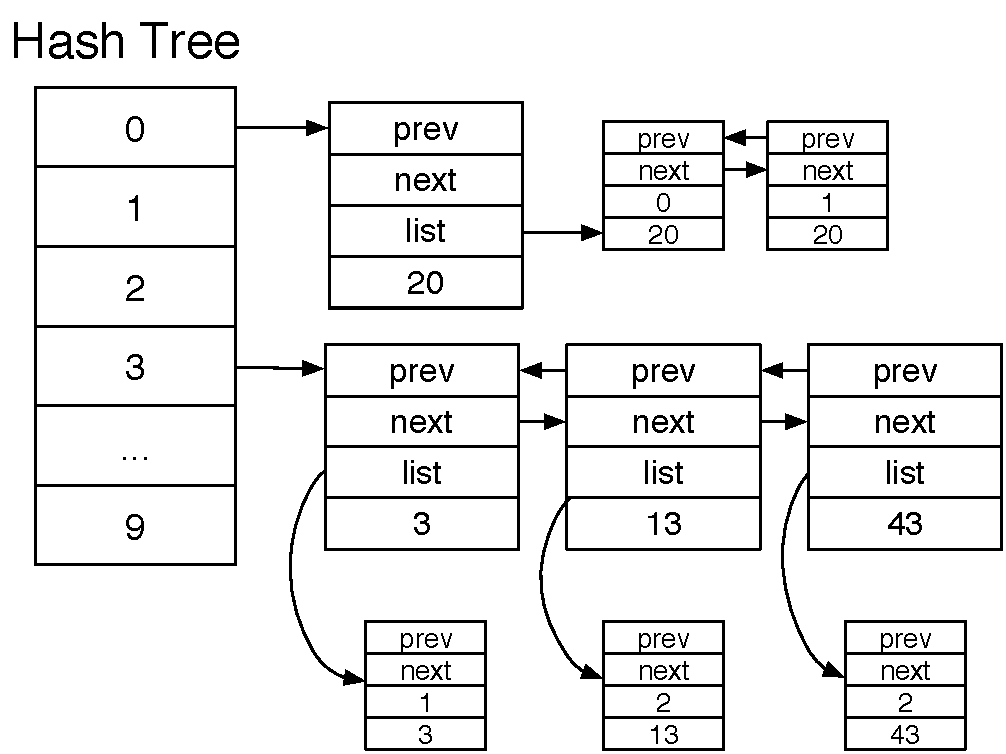
\includegraphics[width=0.6\textwidth]{figures/implementation/hash_table.pdf}
\caption{Hash table and doubly linked data structures for 
   a \texttt{a(int,int)} predicate.}
\label{fig:implementation:hash_table}
\end{figure}

\subsubsection{Locking}

Each node is protected by a main spin-lock that allows threads to change node
attributes. There is also a database spin-lock that protects the internal
database of the node and is locked whenever the node is in the \textbf{working}
state.  

To avoid unnecessary copying, when a node sends facts to a node located in
another thread, the current thread first attempts to lock the database lock of
the target node in order to directly update its database and indexing
structures, otherwise it adds the facts to the list of incoming facts that are
later processed by the owner thread of the target node.


%%%%%%%%%%%%%%%%%%%%%%%%%%%%%%%%%%%%%%%%%%%%%%%%%%%%%%%%%%%%%%%%%%%%%%

\subsection{Rule Engine}
\label{sec:implementation:rule_engine}

The rule engine decides which rules may need to be executed while taking into
account rule priorities. To understand how our engine works, consider the
following set of facts and rules:

\begin{Verbatim}[numbers=left]
a, e(1) -o b.  // rule 1
a -o c.        // rule 2
b -o d.        // rule 3
e(0) -o f.     // rule 4
c -o e(1).     // rule 5

a.
e(0).
\end{Verbatim}

Figure~\ref{fig:implementation:rule_engine} shows the rule engine data
structures for this example. The purpose of each data structure is as follows:

\begin{itemize}

   \item \texttt{Rule Queue} is the bitmap representing the rules scheduled to
      run. The $i^{th}$ is set if the $i^{th}$ rule is scheduled to run;

   \item \texttt{Rule Counter}, which keeps a count of the number of predicates
      needed by the rule that exist in the database. For the rule
      \texttt{a, e(1) -o b} then the rule needs predicates \texttt{a} and
      \texttt{e} and the rule counter is at the most 2 (where the rule can be
      executed).

   \item \texttt{Predicate Bitmap} is a bitmap representing the existence of a
      given predicate in the database;

\end{itemize}

\begin{figure}[t]
   \centering
   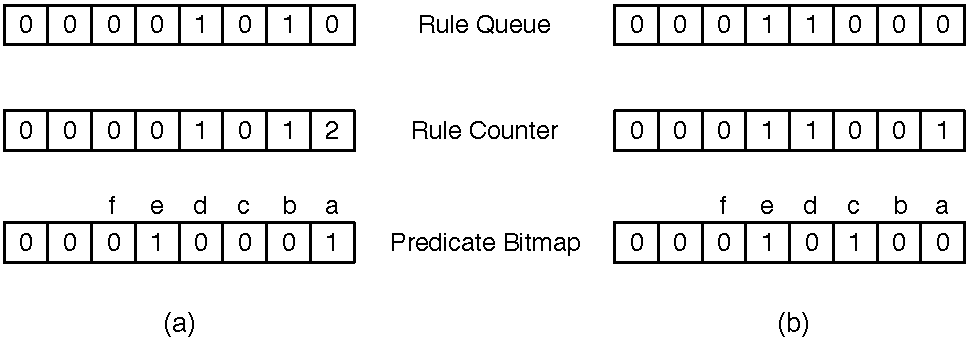
\includegraphics[width=0.8\textwidth]{figures/implementation/rule_queue.pdf}
   \caption{Rule engine data structures (a) before and (b) after applying 
      the rule \texttt{a -o c}.}
   \label{fig:implementation:rule_engine}
\end{figure}

Since we have facts for predicates \texttt{a} and \texttt{e}, the \texttt{Rules
Counter} starts with rules 1, 2 and 4 with 2, 1, 1 predicate counts. Since these
rules have the required counter to be applied, the \texttt{Rule Queue} bitmap
starts with the same three rules.  In order to pick rules for execution, we take
the rule corresponding to the least significant bit from the \texttt{Rule Queue}
bitmap, initially the first rule \texttt{a, e(1) -o b}. However, since we don't
have fact \texttt{e(1)}, this rule fails and its bit in \texttt{Rule Queue} must
be set to 0.  Figure~\ref{fig:implementation:rule_engine}(a) shows the rule
engine data structures at that point.

The next rule in \texttt{Rule Queue} is the second rule \texttt{a -o c}.
Because the this rule will succeed, we must consume fact \texttt{a} and derive
fact \texttt{c}. We thus update \texttt{Predicates Bitmap} accordingly, decrease
the counters for the first and second rule in \texttt{Rule Counter} since such
rules are no longer applicable (\texttt{a} was consumed), and increase the
counter for the fifth rule since \texttt{c} was derived. Finally, to update the
\texttt{Rule Queue}, we must schedule the fifth rule since its counter has been
increased to the required number (we have all predicates).  In the continuation,
the rule engine will schedule the fourth and fifth rules to run.
Figure~\ref{fig:implementation:rule_engine}(b) shows the rule engine data
structures at that point.

Note that every node in the program has the same set of data structures
presented in Fig.~\ref{fig:implementation:rule_engine}. We use 64 bit integers
to implement the 2 bitmaps and an array of 16 bits integers for \texttt{Rule
Counter}.

We do a small optimization to reduce the number of derivations of persistent
facts and, for that, we divide the program rules into two sets: \emph{persistent
rules} and \emph{non persistent rules}. Persistent rules are rules where only
persistent facts are involved. We compile such rules incrementally, i.e., we
attempt to fire all rules where a persistent fact is used. This is called the
\emph{pipelined semi-naive} evaluation and it originated in the P2
system~\cite{Loo-condie-garofalakis-p2}. This evaluation method avoids excessing
re-derivations of the same fact. The order of derivation does not matter for
those rules, since only persistent facts are used.

\subsection{Indexing}\label{sec:implementation:indexing}

To improve fact lookup, the VM employs a fully dynamic mechanism to
decide which argument may be optimal to index.  The algorithm is
performed in the beginning of execution and empirically tries to
assess the argument of each predicate that more equally spreads the
database across the values of the argument.  A single thread performs
the algorithm for all predicates.

The indexing algorithm is performed in three main steps. First, it
gathers lookup statistics by keeping a counter for each
predicate's argument.  Every time a fact search is performed where
arguments are fixed to a value, the counter of such arguments is
incremented. This phase is performed during rule execution for a small
fraction of the nodes in the program.

The second step of the algorithm selects the candidate arguments of each
predicate.  If a predicate was not searched with any fixed arguments, then it
will be not indexed and there are no candidates.  If only one argument was
fixed, then such argument is the only available candidate argument and thus
immediatelly becomes the indexing argument. Otherwise, the top 2 arguments are
selected for the third phase, where \emph{entropy statistics} are collected
dynamically.

During the third phase, each candidate argument has an entropy score.
Before a node is executed, the facts of the target predicate
are used in the following formula applied for the two arguments:

\[
Entropy(A, F) = - \sum_{v \in values(F, A)} \frac{count(F, A = v)}{total(F)} \log_2 \frac{count(F, A = v)}{total(F)}
\]

\noindent where $A$ is the target argument, $F$ is the set of linear facts for
the target predicate, $values(F, A)$ is set of values of the argument $A$,
$count(F, A = v)$ counts the number of linear facts where argument $A$ is equal
to $v$ and $total(F)$ counts the number of linear facts in $F$.  The entropy
value is a good metric because it tells us how much information is needed to
describe an argument. If more information is needed, then that must be the best
argument to index.

For one of the arguments to score, $Entropy(A, F)$ multiplied by the number of
times it has been used for lookup, must be larger than the other argument. The
argument with the best score is selected and then a global variable called
\texttt{indexing\_epoch} is updated. In order to convert the node's linked lists
into hash tables, each node also has a local variable called
\texttt{indexing\_epoch} that is compared to the global variable in order to
rebuild the database according to the new indexing information.

The VM also dynamically resizes the hash table if necessary. When the hash table
becomes too dense, it is doubled in size. When it becomes too sparse, it is
reduced in half or simply transformed back into a doubly linked list. This is
done once in a while, before a node executes.

We have seen very good results with this scheme. The overhead of dynamic
indexing is negligible since programs run almost as fast as if the indices have
been added from the start. However, the programmer can still index predicates
statically, if needed.


\section{Compilation}
As an intermediate step, our compiler first transforms rules into high level
instructions that are then transformed into C++. In Appendix~\ref{appendix:vm}
we present an overview of the high level instructions that can be used as a
reference to the operations that are required by the compiler. In this section,
we present the main algorithm of the compiler and its key optimizations. To make
our presentation more readable, we present our examples using pseudo-code
instead of C++ code.

\subsection{Ordinary Rules}\label{sec:compile}

After a rule is compiled, it must respect the \emph{fact constraints}
(facts must exist in the database) and the \emph{join constraints} that can be
represented by variable constraints and/or boolean expressions. For instance,
consider the second rule of the bipartiteness checking program presented in
Fig.~\ref{language:code:bichecking}:

\begin{Code}
visit(A, P),
colored(A, P)
   -o colored(A, P).
\end{Code}

The fact constraint include the facts required to trigger the rule, namely
\code{visit(A, P)} and \code{colored(A, P)}, and the join constraints include
the implicit constraint that the second argument of \code{visit} must be equal
to the second argument of \code{colored} because the variable \code{P} is used
for both arguments. However, rules may also have explicit constraints, such as:

\begin{Code}
visit(A, P1),
colored(A, P2),
P1 <> P2
   -o fail(A).
\end{Code}

The data structures presented in Section~\ref{sec:data_structures} support
iteration over facts and for linear facts, they also support deletion. Iteration
is provided through \emph{iterators}. For linked lists, the iterator points to
the linear fact in the list and uses the \code{next} field to traverse the list.
For hash tables, it is possible to iterate through the whole table or iterate
through a single bucket. For tries, while iteration goes through every fact, the
operation can be customized with join constraints in order to prune search. To
illustrate how rules are compiled, consider again the rule:

\begin{Code}
visit(A, P),
colored(A, P)
   -o colored(A, P).
\end{Code}

The compiler transforms the rule into two nested \emph{while} loops, as follows:

\begin{LineCode}
colored_list <- linked_list("colored")
visit_list <- linked_list("visit")
visit <- visit_list.head()
while(visit is valid)
{
   colored <- colored_list.head() // Retrieve first element of the list.
   while(colored is valid)
   {
      if(visit.get_int(1) == colored.get_int(1)) { // Equal arguments?
         // New fact is derived.
         new_colored <- create_fact("colored") // New fact for predicate colored.
         new_colored.set_int(1, visit.get_int(1)) // Set arguments.

         colored_list.add(new_colored) // Add new fact to the linked list.

         // Deleting used up facts.
         colored <- colored_list.delete_and_next(colored)
         visit <- visit_list.delete_and_next(visit)
         goto next
      }
      colored <- colored.next()
   }
   visit <- visit.next()
next:
   continue
}
\end{LineCode}

The compilation algorithm iterates through the atomic propositions of the rule's
LHS and creates nested loops to try all the possible combinations of facts.  For
this rule, all the pairs of facts \code{colored} and \code{visit} must be
searched until the implicit constraint is true. First, the \code{visit} linked
list is iterated over by first retrieving the head fact and then using the
\code{next} pointer of each fact. Inside this outer loop, a nested \code{while}
loop is created for predicate \code{colored}. This inner loop includes a check
for the constraint.

If the constraint expression is true then the rule matches and a new
\code{colored} fact is derived and two used linear facts are consumed by
deleting them from the linked lists. After the rule is derived, the \code{visit}
and \code{colored} facts are deleted from the linked list and the pointers
adjusted to the next elements of each list. Afterwards, the \code{goto next}
statement is used to jump to the outer loop, which will use the new fact
pointers. This forces the procedure to try all the combinations of the rule from
the database.  Furthermore, we must jump to the first linear loop because we
cannot use the next fact from the deepest loop since we may have constraints
between the first linear loop and the deepest loop that were validated using
deleted facts.

If the implicit constraint failed, another \code{colored} fact would be checked
by assigning \code{colored} to \code{colored.next()}.  Likewise, if the initial
\code{visit} fact fails for all \code{colored} facts, then the next
\code{visit} fact in the list is tried by following the \code{next} pointer.

In order to understand how rule priorities affect compilation, consider a
slightly different bipartiteness checking program where the second and third
rules are swapped:

\begin{LineCode}[commandchars=\*\[\]]
visit(A, P),
uncolored(A)
   -o {B | !edge(A, B) -o visit(B, next(P))},
      colored(A, P).

visit(A, P1),
colored(A, P2),
P1 <> P2
   -o fail(A).*label[line:implementation:higher]

*textbf[visit(A, P),]
*textbf[colored(A, P)]
   *textbf[-o colored(A, P).]

visit(A, P),
fail(A)
   -o fail(A).
\end{LineCode}

The procedure for the rule being compiled cannot be the same since the derived
\code{colored} fact is used in the LHS of a higher priority rule, namely, the
rule in line~\ref{line:implementation:higher}. Once the \code{colored} fact is
derived, the procedure must return to schedule the higher priority rule, as
follows:

\begin{LineCode}[commandchars=\$\#\&]
colored_list <- linked_list("colored")
visit_list <- linked_list("visit")
colored <- colored_list.head()
while(colored is valid)
{
   visit <- visit_list.head() // Retrieve first element of the list.
   while(visit is valid)
   {
      if(visit.get_int(1) == colored.get_int(1)) { // Equal arguments?
         new_colored <- create_fact("colored") // New fact for predicate colored.
         new_colored.set_int(1, visit.get_int(1)) // Set arguments.

         // New fact is derived.
         colored_list.add(new_colored) // Add new fact to the linked list.

         // Deleting facts.
         colored_list.delete_and_next(colored)
         visit_list.delete_and_next(visit)
         $textbf#return&
      }
      visit <- visit.next()
   }
   colored <- colored.next()
}
\end{LineCode}

This enforces the priority semantics of the language described in
Section~\ref{sec:language:semantics}. When a rule derives facts
that were used as input to a higher priority rule, the initial rule is only
derived once because the newly derived facts may trigger the derivation of a
higher priority rule.
    
\begin{figure}
\begin{algorithm}[H]
 \KwData{Rule R1, Rules}
 \KwResult{Compiled Code}
 $LHSProps \longleftarrow LHSAtomicPropositionsFromRule(R1)$\;
 $Constraints \longleftarrow ConstraintsFromRule(R1)$\;
 $Code \longleftarrow CreateFunctionForRule()$\;
 $FactIterators \longleftarrow []$\;
 $CompiledProps = []$\;
 \While{$LHSProps$ not empty}{
  $Prop \longleftarrow RemoveBestProposition(LHSProps)$\;
  $CompiledProps.push(Prop)$\;
  $Iterator \longleftarrow Code.InsertIteration(Prop)$\;
  $FactIterators.push(Iterator)$\;
  \tcp{Select constraints that are covered by CompiledFacts.}
  $NextConstraints \longleftarrow RemoveConstraints(Constraints, CompiledProps)$\;
  $Code.InsertConstraints(NextConstraints)$\;
 }
 $RHSProps = RHSAtomicPropositionsFromRule(R1)$\;
 \While{$RHSProps$ not empty}{
    $Prop \longleftarrow RemoveFact(RHSProps)$\;
    $Code.InsertDerivation(Prop)$\;
 }
 \For{$Iterator \in FactIterators$}{
    \If{$IsLinear(Iterator)$}{
       $Code.InsertRemove(Iterator)$\;
    }
 }
 \tcp{Enforce rule priorities.}
 \uIf{$FactsDerivedUsedBefore(Rules, R1)$}{
    $Code.InsertReturn()$\;
 }
 \Else{
    $Code.InsertGoto(FirstLinear(FactIterators))$\;
 }
 \Return{$Code$}
\end{algorithm}
 \mycap{Compiling LM rules into C++ code.}
 \label{alg:compile_rule}
\end{figure}

Figure~\ref{alg:compile_rule} presents the algorithm for compiling rules into
C++ code. First, we split the rule's RHS into atomic propositions and
constraints. Fact expressions map directly to iterators while fact constraints
map to \emph{if} expressions. A possible compilation strategy is to first
compile all the atomic propositions and then compile the constraints. However,
this may require unneeded database lookups since some constraints may fail
early.  Therefore, our compiler introduces constraints as soon as all the
variables in the constraint are all included in the already compiled atomic
propositions. The order in which fact propositions are selected for compilation
does not interfere with the correctness of the compiled code, thus our compiler
selects the atomic proposition ($RemoveBestProposition$) that needs the highest
number of join constraints, in order to prune search and avoid undesirable
database lookups. If two atomic propositions have the same number of new
constraints, then the compiler always picks the persistent proposition since
persistent facts are not deleted.

Derivation of new facts belonging to the local node requires only that the new
facts are added to the local node data structure. Facts that belong to other
nodes are sent using an appropriate runtime API.

\subsection{Persistence Checking}

Not all linear facts need to be deleted. For instance, in the compiled rule
above, the fact \code{colored(A, P)} is re-derived in the rule's RHS.  Our
compiler is able to turn linear loops into persistent loops for linear facts
that are consumed and then asserted. The rule is then compiled as follows:

\begin{LineCode}[commandchars=\$\#\&]
colored_list <- linked_list("colored")
visit_list <- linked_list("visit")
colored <- colored_list.head()
while(colored is valid)
{
   visit <- visit_list.head() // Retrieve first element of the list.
   while(visit is valid)
   {
      if(visit.get_int(1) == colored.get_int(1)) { // Equal arguments?
         // Delete visit.
         visit <- visit_list.delete_and_next(visit) // Get next visit fact.
         goto next$label#line:implementation:goto&
      }
      visit <- visit.next()
$textbf#next:&
      $textbf#continue&
   }
   colored <- colored.next()
}
\end{LineCode}

In this new version of the code, only the \code{visit} facts are deleted, while
the \code{colored} facts remain untouched. In the bipartiteness checking
program, each node has one \code{colored} fact and this compiled code simply
filters out the \code{visit} facts with the same color. Please note that the
\code{colored} facts are now iterated in the outer loop in order to make the
\code{goto} statement jump to the inner loop. This is now possible because the
\code{colored} fact is not deleted during rule derivation.

\subsection{Updating Facts}

Many inference rules consume and then derive the same predicate but with
different arguments. The compiler recognizes those cases and, instead of
consuming the fact from its linked list or hash table, it updates the fact
in-place. As an example, consider the following rule:

\begin{Code}
new-neighbor-pagerank(A, B, New),
neighbor-pagerank(A, B, Old)
   -o neighbor-pagerank(A, B, New).
\end{Code}

Assuming that \code{neighbor-pagerank} is stored in a hash table and indexed by
the second argument, the code for the rule above is as follows:

\begin{LineCode}
new_neighbor_pagerank_list <- linked_list("new-neighbor-pagerank")
neighbor_pagerank_table <- hash_table("neighbor-pagerank")
new_neighbor_pagerank <- new_neighbor_pagerank.head()
while(new_neighbor_pagerank is valid)
{
   // Hash table for neighbor-pagerank is indexed by the second argument,
   // therefore we search for the bucket using the second argument
   // of new-neighbor-pagerank.
   neighbor_pagerank <- neighbor_pagerank_table.lookup(new_neighbor_pagerank.get_node(1))
   while(neighbor_pagerank is valid)
   {
      if(new_neighbor_pagerank.get_node(1) == neighbor_pagerank.get_node(1))
      {
         // Update fact argument.
         neighbor_pagerank.set_float(2, new_neighbor_pagerank.get_float(2))
         new_neighbor_pagerank <- new_neighbor_pagerank_list.
                  delete_and_next(new_neighbor_pagerank)
         goto next
      }
      neighbor_pagerank <- neighbor_pagerank.next()
   }
   new_neighbor_pagerank <- new_neighbor_pagerank.next()
next:
   continue
}
\end{LineCode}

Note that \code{neighbor-pagerank} fact is updated using \code{set\_float}. The
rule also does not return since it is the highest priority rule. If there was a
higher priority rule using \code{neighbor-pagerank}, then the code would have to
return since the act of updating a fact is equivalent to deriving a new one.

\subsection{Enforcing Linearity}

We have already introduced the \code{goto} statement as a mechanism to avoid
reusing deleted linear facts. However, this is not enough in order to enforce
linearity of facts. Consider the following inference rule:

\begin{Code}
add(A, N1),
add(A, N2)
   -o add(A, N1 + N2).
\end{Code}

Using the standard compilation algorithm, two nested loops are created, one for
each \code{add} fact. However, notice that there is an implicit constraint (the
two \code{add} linear facts must be different) when creating the iterator for
\code{add(A, N2)} since this fact cannot be the same as the first one. That
would invalidate linearity since a single linear fact would be used to prove two
linear facts. This is easily solved by adding a constraint in the inner loop by
checking if the second fact is the same as the first one.

\begin{LineCode}
add_list <- linked_list("add")
add1 <- add_list.head()
while(add1 is valid)
{
   add2 <- add_list.head()
   while(add2 is valid)
   {
      if(add1 != add2)
      {
         add1.set_int(1, add1.get_int(1) + add2.get_int(1))
         add2 <- add_list.delete_and_next(add2)
         goto next
      }
      add2 <- add2.next()
   }
   add1 <- add1.next()
next:
   continue
}
\end{LineCode}

Figure~\ref{fig:local:update_add} presents the steps for executing this rule
when the database contains three facts. The fact variables never point to the
same fact.

\begin{figure}
\centering
\begin{minipage}{.5\textwidth}
  \centering
  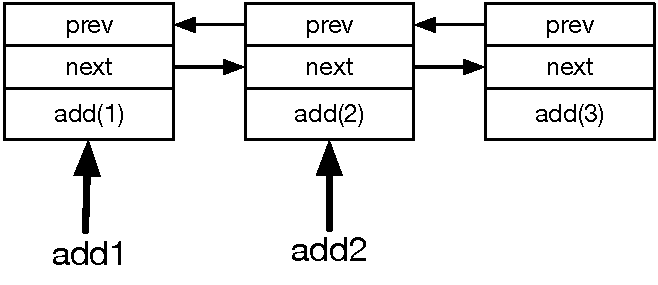
\includegraphics[width=.8\linewidth]{figures/compiler/update}
\end{minipage}%
\begin{minipage}{.5\textwidth}
  \centering
  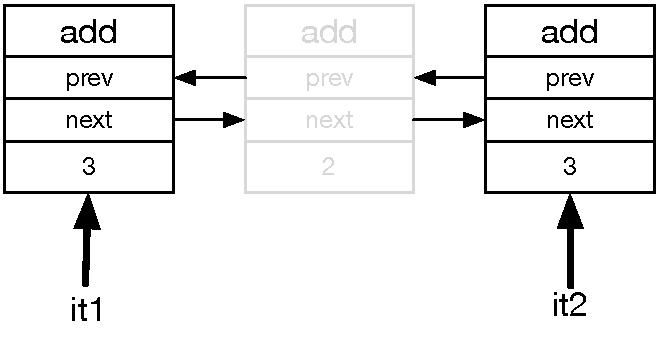
\includegraphics[width=0.8\linewidth]{figures/compiler/update2}
\end{minipage}
\begin{minipage}{.5\textwidth}
   \centering
   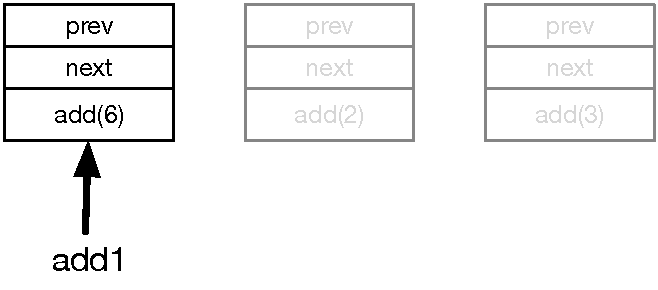
\includegraphics[width=0.8\linewidth]{figures/compiler/update3}
\end{minipage}
\mycap{Executing the add rule. First, the two iterators point to
   the first and second facts and the former is updated while the latter is
   consumed. The second iterator then moves to the next fact and the first fact is
   updated again, now to the value \code{6}, the expected result.}
\label{fig:local:update_add}
\end{figure}

\subsection{Comprehensions}

Consider the comprehension used in the first rule of the bipartiteness checking
program in Fig.~\ref{language:code:bichecking}:

\begin{Code}
visit(A, P),
uncolored(A)
   -o {B | !edge(A, B) -o visit(B, next(P))},
      colored(A, P).
\end{Code}

The attentive reader will remember that comprehensions are sub-rules, therefore
they should be compiled like normal rules. Comprehensions must also derive all
possible combinations. However, the rule itself must return if the
comprehension's RHS derives a fact that is used by a higher priority rule. The
example rule does not need to return since it has the highest priority and the
\code{visit} facts derived in the comprehension are contained in other nodes.
The code for the rule is shown below:

\begin{LineCode}
colored_list <- linked_list("colored")
visit_list <- linked_list("visit")
uncolored_list <- linked_list("uncolored")
visit <- visit_list.head()
while(visit is valid)
{
   uncolored <- uncolored_list.head()
   while(uncolored is valid)
   {
      // Comprehension code.
      edge_trie <- trie("edge")
      edge <- edge_trie.first()
      while(edge is valid)
      {
         new_visit <- create_fact("visit") // New visit fact.
         new_visit.set_int(1, next(visit.get_int(1)))
         // Send fact to B.
         send_fact(new_visit, edge.get_node(1))
         edge <- edge.next()
      }
      new_colored <- create_fact("colored")
      new_colored.set_int(1, visit.get_int(1))
      colored_list.add(new_colored)
      visit <- visit_list.delete_and_next(visit)
      uncolored <- uncolored_list.delete_and_next(uncolored)
      goto next
   }
   uncolored <- uncolored.next()
next:
   continue
}
\end{LineCode}

Special care must be taken when the comprehension's sub-rule uses the same
predicates that are derived by the main rule. Rule inference must be atomic in
the sense that, after a rule matches, the comprehensions in the rule's RHS can
use the facts that were present before the rule was matched. Consider a rule
with $n$ comprehensions or aggregates, where each $CLHS_i$ and $CRHS_i$ are the
LHS and RHS of the comprehension/aggregate $i$, respectively, and $RHSP$
represents the atomic propositions found in rule's RHS. The formula used by the
compiler to detect conflicts between predicates is the following:

\[
\bigcup^{n}_i[CLHS_i \cap RHSP] \cup \bigcup^{n}_i [CLHS_i \cap \bigcup^{n}_j[CRHS_j]]
\]

If the result of the formula is not empty, then the compiler disables
optimizations for the conflicting predicates and derives the corresponding facts
into a temporary data structure before being added into the database data
structures. As an example, consider the following rule:

\begin{Code}
update(A),
!edge(A, B)
   -o {P | points(A, B, P) -o update(B)},
      points(A, B, 1).
\end{Code}

We have $n = 1$ comprehensions, where $CLHS_0 = $ \code{points(A, B, P)},
$CRHS_0 =$ \code{update(B)}, and $RHSP = $ \code{points(A, B, 1)}. There is a
conflict because $CLHS_0 \cap RHSP = \{\mathtt{points}\}$, which requires
\code{points(A, B, 1)} to be derived after the comprehension or be stored in a
temporary data structure to avoid conflicts with the comprehensions, which could
consume the newly derived fact. Fortunately, most rules in LM programs do not
show these kinds of conflicts and thus can be fully optimized.

\subsection{Aggregates}

Aggregates are similar to comprehensions. They are also sub-rules but a value is
accumulated for each combination of the sub-rule. After all the combinations are
derived, a final RHS term is derived with the accumulated value. Consider the
following rule that computes a PageRank value by aggregating all neighbors
PageRank values:

\begin{Code}
update(A),
pagerank(A, OldRank)
      -o [sum => V; B | neighbor-pagerank(A, B, V) -o neighbor-pagerank(A, B, V)
            -> pagerank(A, damping/P + (1.0 - damping) * V)].
\end{Code}

The variable \code{V} is initialized to \code{0.0} and sums all the PageRank
values of the neighbors as seen in the code below. The aggregate value is then
used to update the second argument of the initial \code{pagerank} fact.

\begin{LineCode}
pagerank_list <- linked_list("pagerank")
update_list <- linked_list("update")
neighbor_pagerank_list <- linked_list("neighbor_pagerank_list")
pagerank <- pagerank_list.head()
while(pagerank is valid)
{
   update <- update_list.head()
   while(update is valid)
   {
      V <- 0.0
      neighbor_pagerank <- neighbor_pagerank_list.head()
      while(neighbor_pagerank is valid)
      {
         V <- V + neighbor_pagerank.get_float(2)
         neighbor_pagerank <- neighbor_pagerank.next()
      }
      // RHS of the aggregate
      pagerank.set_float(1, damping / P + (1.0 - damping) * V)
      update <- update_list.delete_and_next(update)
      goto next
   }
   pagerank <- pagerank.next()
next:
   continue
}
\end{LineCode}



\section{Summary}

This section provided a full description of the implementation of LM, including
its compiler and virtual machine. We explained how the virtual machine is
organized to provide scalable multi threaded execution and fast fact assertion
and retraction using efficient data structures. We also gave a detailed
description of the compilation algorithm used to transform LM rules into
efficient C++ code.
